\documentclass[11pt]{article}

\newcommand{\yourname}{}
\newcommand{\yourcollaborators}{}

\def\comments{0}

%format and packages

%\usepackage{algorithm, algorithmic}
\usepackage{algpseudocode}
\usepackage{amsmath, amssymb, amsthm}
\usepackage{enumerate}
\usepackage{enumitem}
\usepackage{framed}
\usepackage{verbatim}
\usepackage[margin=1.0in]{geometry}
\usepackage{microtype}
\usepackage{kpfonts}
\usepackage{graphicx}       % upload image
\usepackage{palatino}
	\DeclareMathAlphabet{\mathtt}{OT1}{cmtt}{m}{n}
	\SetMathAlphabet{\mathtt}{bold}{OT1}{cmtt}{bx}{n}
	\DeclareMathAlphabet{\mathsf}{OT1}{cmss}{m}{n}
	\SetMathAlphabet{\mathsf}{bold}{OT1}{cmss}{bx}{n}
	\renewcommand*\ttdefault{cmtt}
	\renewcommand*\sfdefault{cmss}
	\renewcommand{\baselinestretch}{1.06}
\usepackage[usenames,dvipsnames]{xcolor}
\definecolor{DarkGreen}{rgb}{0.15,0.5,0.15}
\definecolor{DarkRed}{rgb}{0.6,0.2,0.2}
\definecolor{DarkBlue}{rgb}{0.2,0.2,0.6}
\definecolor{DarkPurple}{rgb}{0.4,0.2,0.4}
\usepackage[pdftex]{hyperref}
\hypersetup{
	linktocpage=true,
	colorlinks=true,				% false: boxed links; true: colored links
	linkcolor=DarkBlue,		% color of internal links
	citecolor=DarkBlue,	% color of links to bibliography
	urlcolor=DarkBlue,		% color of external links
}

\usepackage[boxruled,vlined,nofillcomment]{algorithm2e}
	\SetKwProg{Fn}{Function}{\string:}{}
	\SetKwFor{While}{While}{}{}
	\SetKwFor{For}{For}{}{}
	\SetKwIF{If}{ElseIf}{Else}{If}{:}{ElseIf}{Else}{:}
	\SetKw{Return}{Return}
	

%enclosure macros
\newcommand{\paren}[1]{\ensuremath{\left( {#1} \right)}}
\newcommand{\bracket}[1]{\ensuremath{\left\{ {#1} \right\}}}
\renewcommand{\sb}[1]{\ensuremath{\left[ {#1} \right\]}}
\newcommand{\ab}[1]{\ensuremath{\left\langle {#1} \right\rangle}}

%probability macros
\newcommand{\ex}[2]{{\ifx&#1& \mathbb{E} \else \underset{#1}{\mathbb{E}} \fi \left[#2\right]}}
\newcommand{\pr}[2]{{\ifx&#1& \mathbb{P} \else \underset{#1}{\mathbb{P}} \fi \left[#2\right]}}
\newcommand{\var}[2]{{\ifx&#1& \mathrm{Var} \else \underset{#1}{\mathrm{Var}} \fi \left[#2\right]}}

%useful CS macros
\newcommand{\poly}{\mathrm{poly}}
\newcommand{\polylog}{\mathrm{polylog}}
\newcommand{\zo}{\{0,1\}}
\newcommand{\pmo}{\{\pm1\}}
\newcommand{\getsr}{\gets_{\mbox{\tiny R}}}
\newcommand{\card}[1]{\left| #1 \right|}
\newcommand{\set}[1]{\left\{#1\right\}}
\newcommand{\negl}{\mathrm{negl}}
\newcommand{\eps}{\varepsilon}
\DeclareMathOperator*{\argmin}{arg\,min}
\DeclareMathOperator*{\argmax}{arg\,max}
\newcommand{\eqand}{\qquad \textrm{and} \qquad}
\newcommand{\ind}[1]{\mathbb{I}\{#1\}}
\newcommand{\sslash}{\ensuremath{\mathbin{/\mkern-3mu/}}}

%mathbb
\newcommand{\N}{\mathbb{N}}
\newcommand{\R}{\mathbb{R}}
\newcommand{\Z}{\mathbb{Z}}
%mathcal
\newcommand{\cA}{\mathcal{A}}
\newcommand{\cB}{\mathcal{B}}
\newcommand{\cC}{\mathcal{C}}
\newcommand{\cD}{\mathcal{D}}
\newcommand{\cE}{\mathcal{E}}
\newcommand{\cF}{\mathcal{F}}
\newcommand{\cL}{\mathcal{L}}
\newcommand{\cM}{\mathcal{M}}
\newcommand{\cO}{\mathcal{O}}
\newcommand{\cP}{\mathcal{P}}
\newcommand{\cQ}{\mathcal{Q}}
\newcommand{\cR}{\mathcal{R}}
\newcommand{\cS}{\mathcal{S}}
\newcommand{\cU}{\mathcal{U}}
\newcommand{\cV}{\mathcal{V}}
\newcommand{\cW}{\mathcal{W}}
\newcommand{\cX}{\mathcal{X}}
\newcommand{\cY}{\mathcal{Y}}
\newcommand{\cZ}{\mathcal{Z}}

%theorem macros
\newtheorem{thm}{Theorem}
\newtheorem{lem}[thm]{Lemma}
\newtheorem{fact}[thm]{Fact}
\newtheorem{clm}[thm]{Claim}
\newtheorem{rem}[thm]{Remark}
\newtheorem{coro}[thm]{Corollary}
\newtheorem{prop}[thm]{Proposition}
\newtheorem{conj}[thm]{Conjecture}

\theoremstyle{definition}
\newtheorem{defn}[thm]{Definition}


\newcommand{\instructor}{Virgil Pavlu}
\newcommand{\hwnum}{10}
\newcommand{\hwdue}{Wednesday, May 20 at 11:59pm via \href{https://gradescope.com/courses/229309}{Gradescope}}

\theoremstyle{theorem}
\newtheorem{prob}{}
\newtheorem{sol}{Solution}

\definecolor{cit}{rgb}{0.05,0.2,0.45} 
\newcommand{\solution}{\medskip\noindent{\color{DarkBlue}\textbf{Solution:}}}

\begin{document}
{\Large 
\begin{center}{CS5800: Algorithms} --- Spring '21 --- \instructor \end{center}}
{\large
\vspace{10pt}
\noindent Homework~\hwnum \vspace{2pt}\\
Submit via \href{https://www.gradescope.com/courses/232127}{Gradescope}}

\bigskip
{\large \noindent Name: Xuran Feng }

{\large \noindent Collaborators: \yourcollaborators}

\vspace{15pt}

{\large \noindent Instructions:}

\begin{itemize}

\item Make sure to put your name on the first page.  If you are using the \LaTeX~template we provided, then you can make sure it appears by filling in the \texttt{yourname} command.

\item Please review the grading policy outlined in the course information page.

\item You must also write down with whom you worked on the assignment.  If this changes from problem to problem, then you should write down this information separately with each problem.

\item Problem numbers (like Exercise 3.1-1) are corresponding to CLRS $3^{rd}$ edition.  While the  $2^{nd}$ edition  has  similar  problems  with  similar  numbers,  the  actual  exercises  and their solutions are different, so make sure you are using the $3^{rd}$ edition.

\end{itemize}

\newpage

\begin{prob} \textbf{(15 points)} Exercise 22.1-5.
\end{prob}
\solution
For each vertex v, iterate all neighbours, and for each neighbour n of v, mark all neighbours of n for v. It's like doing BFS of each vertex but with a limit to 2 waves.\\
For each vertex v of G:\\
\null\qquad for each neighbour n1 of v:\\
\null\qquad\qquad mark edge(v, n1)\\
\null\qquad\qquad for each neighbour n2 of n1:\\
\null\qquad\qquad\qquad mark edge(v, n2)\\
The running time of the graph square using adjacency matrix is $O(V^3)$ because we need to traverse neighbour of neighbour of each vertex; the running time of the graph square using adjacency list is $O(|V||E|)$ because for each vertex we may need to go through every edge.
\begin{prob} \textbf{(15 points)} Exercise 22.2-6.
\end{prob}
\solution\\
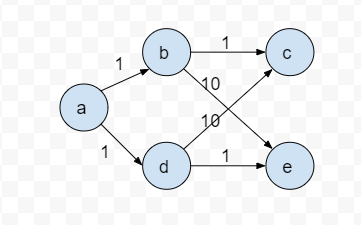
\includegraphics[width=8cm, height=5cm]{1}
\\A valid set of tree edges are edge(a,b), edge(a,d), edge(b,c) and edge(d,e). This is why BFS fails to find shortest path when edges have weights. From the graph above, if starting from vertex a, the first wave of BFS will add b and d into the queue and edge(a,b) and edge(a,d) will be employed; however when b gets popped, edge(b,c) and edge(b,e) will be employed, c and e are added into the queue; when d gets popped, edge(d,c) and edge(d,e) will never be considered because c and e are already added to the queue. The problem is edge(b,c) and edge(d,e) are for sure the shortest path to c and e respectively but BFS will not employ edge(b,c) and edge(d,e) at the same time because edge(b,e) must be employed with edge(b,c) together, edge(d,c) and edge(d,e) must be employed together. So BFS can never produce a tree like this.\\
\begin{prob} \textbf{(15 points)} Exercise 22.2-7.
\end{prob}
\solution
We can see all the wrestlers as vertex and the pair relation as an edge, so now a tree has been formed. Then we can do BFS search, we randomly start from a vertex and assign a number A to it meaning this vertex is already a babyface or heel, then mark this vertex as visited, for all neighbours of this vertex, assigning a number B to each meaning the neighbours must be in different parties and add each neighbour to the queue. Continuing the BFS, when a node n gets dequeued, for all neighbours of this node, if the neighbour already has a number and the number is same as n's number, return false; else if the neighbour's number is different from n's, continue checking other neighbours; else assign an opposite number to its neighbour and enqueue this neighbour.\\
BFS(G,s)\\
\null\qquad for each vertex u:\\
\null\qquad\qquad u.visited=false\\
\null\qquad s.Number=A\\
\null\qquad ENQUEUE(Q,s)\\
\null\qquad while(Q.size$>$0)\\
\null\qquad\qquad u=DEQUEUE(Q)\\
\null\qquad\qquad for(each v that belongs to G.Adj[u])\\
\null\qquad\qquad\qquad if v.visited=true then continue;\\
\null\qquad\qquad\qquad if v.number!=null and v.number==u.number\\
\null\qquad\qquad\qquad\qquad return false;\\
\null\qquad\qquad\qquad if v.number!=null and v.number!=u.number\\
\null\qquad\qquad\qquad\qquad continue;\\
\null\qquad\qquad\qquad assign an opposite number to v\\
\null\qquad\qquad\qquad ENQUEUE(v)\\
\null\qquad\qquad u.visited=true\\
The running time of this algorithm is O(n+r) because it is a modified algorithm based on BFS and BFS has a time complexity of O(n+r).
\begin{prob} \textbf{(10 points)} Exercise 22.3-7.
\end{prob}
\solution\\
DFS(G)\\
\null\qquad for each vertex u:\\
\null\qquad\qquad u.color=WHITE\\
\null\qquad\qquad u.p=NIL\\
\null\qquad time=0\\
\null\qquad stack=\{\}\\
\null\qquad for each vertex u:\\
\null\qquad\qquad if u.color==WHITE\\
\null\qquad\qquad\qquad stack.PUSH(u)\\
\null\qquad\qquad\qquad DFS-VISIST(G,stack)\\
DFS-VISIT(G,stack)\\
\null\qquad u.d=++time\\
\null\qquad u.color=GRAY\\
\null\qquad while(stack.size$>$0)\\
\null\qquad\qquad u=stack.peek()\\
\null\qquad\qquad while(u.hasWhiteNeighbour()):\\
\null\qquad\qquad\qquad v=u.getWhiteNeighbour()\\
\null\qquad\qquad\qquad v.d=++time\\
\null\qquad\qquad\qquad v.color=GRAY\\
\null\qquad\qquad\qquad v.p=u\\
\null\qquad\qquad\qquad stack.push(v)\\
\null\qquad\qquad\qquad u=v\\
\null\qquad\qquad u=stack.pop()\\
\null\qquad\qquad u.color=BLACK\\
\null\qquad\qquad u.f=++time\\\\
hasWhiteNeighbour(u)\\
\null\qquad for vertex v that are adjacent to u\\
\null\qquad\qquad if v.color==WHITE\\
\null\qquad\qquad\qquad return true\\
\null\qquad return false\\
getWhiteNeighbour(u)\\
\null\qquad for vertex v that are adjacent to u\\
\null\qquad\qquad if v.color==WHITE\\
\null\qquad\qquad\qquad return v\\
\null\qquad return null\\
\begin{prob} \textbf{(10 points)} Exercise 22.3-10.
\end{prob}
\solution\\
DFS(G)\\
\null\qquad for each vertex u:\\
\null\qquad\qquad u.color=WHITE\\
\null\qquad\qquad u.p=NIL\\
\null\qquad time=0\\
\null\qquad for each vertex u:\\
\null\qquad\qquad if u.color==WHITE\\
\null\qquad\qquad\qquad DFS-VISIST(G,u)\\
DFS-VISIT(G,u)\\
\null\qquad u.d=++time\\
\null\qquad u.color=GRAY\\
\null\qquad for each v that is adjacent to u:\\
\null\qquad\qquad if v.color==WHITE\\
\null\qquad\qquad\qquad v.p=u\\
\null\qquad\qquad\qquad output("tree edge from u to v")\\
\null\qquad\qquad\qquad DFS-VISIT(G,v)\\
\null\qquad\qquad else if v.color==GRAY\\
\null\qquad\qquad\qquad output("back edge from v to u")\\
\null\qquad\qquad else if v.d$>$u.d\\
\null\qquad\qquad\qquad output("forward edge from u to v")\\
\null\qquad\qquad else output("cross edge from u to v")\\
\null\qquad u.color=BLACK\\
\null\qquad u.f=++time\\
If G is undirected, then there is no cross edge because DFS will allow search as far as possible; back edge and forward edge are actually pointing to same edge because the undirected edge can be seen as a bidirectional edge, but the tree edge serves the same function.\\
\begin{prob} \textbf{(15 points)} Exercise 22.3-12.
\end{prob}
\solution\\Because the graph now is undirected, the undirected relation between two vertex can be seen as a bidirectional relation, as long as there is an edge from u to v, then there must be an edge from v to u at the same time. So as long as the DFS can continue going, all vertex that have been traversed must be reachable for each other. However, all vertex may not be connected together, there could be several trees can form a forest, so the total times of running DFS before all vertex are all marked finished means in fact the number of separate trees in this forest.\\
DFS(G)\\
\null\qquad for each vertex u:\\
\null\qquad\qquad u.color=WHITE\\
\null\qquad\qquad u.p=NIL\\
\null\qquad time=0\\
\null\qquad cc=1\\
\null\qquad for each vertex u:\\
\null\qquad\qquad if u.color==WHITE\\
\null\qquad\qquad\qquad u.cc=cc\\
\null\qquad\qquad\qquad DFS-VISIST(G,u)\\
\null\qquad\qquad\qquad cc++\\
DFS-VISIT(G,u)\\
\null\qquad u.d=++time\\
\null\qquad u.color=GRAY\\
\null\qquad for each v that is adjacent to u:\\
\null\qquad\qquad if v.color==WHITE\\
\null\qquad\qquad\qquad v.p=u\\
\null\qquad\qquad\qquad v.cc=u.cc\\
\null\qquad\qquad\qquad DFS-VISIT(G,v)\\
\null\qquad u.color=BLACK\\
\null\qquad u.f=++time
\begin{prob} \textbf{(20 points)} Exercise 22.4-5.
\end{prob}
\solution
Use a queue to continue enquequing vertex that has an in-degree 0(out-degree 1) and every time we dequeue a vertex from the queue, we iterate all its neighbours and decrement neighbour's in-degree by 1, if any neighbour reaches a 0 in-degree, enqueue it. Continue until the queue is empty.\\ 
TopoSort(G)\\
\null\qquad queue=\{\}\\
\null\qquad for each vertex u:\\
\null\qquad\qquad if u.in-degree==0\\
\null\qquad\qquad\qquad queue.ENQUEUE(u)\\
\null\qquad while(queue.size$>$0):\\
\null\qquad\qquad u=queue.DEQUEUE()\\
\null\qquad\qquad for each v that is adjacent to u:\\
\null\qquad\qquad\qquad v.in-degree=v.in-degree - 1\\
\null\qquad\qquad\qquad if v.in-degree==0\\
\null\qquad\qquad\qquad\qquad queue.ENQUEUE(v)\\
Because the iterative TopoSort is actually modified from BFS with just different enqueuing and dequeuing orders, since BFS runs in time O(V+E), this topological sort also runs in O(V+E) time. If G has cycles, this algo will end too early because there are still vertex left to be traversed but since there is a deadlock so no vertex can first reach an in-degree 0 to be enqueued, the queue will become empty while some vertex are still unvisited.\\
\begin{prob} \textbf{(15 points)} Two special vertices $s$ and $t$ in the undirected graph G=(V,E) have the following  property:  any  path  from  $s$  to  $t$  has  at  least  $1  +|V|/2$  edges.   Show  that  all paths from $s$ to $t$ must have a common vertex $v$ (not equal to either $s$ or $t$) and give an algorithm with running time O(V+E) to find such a node $v$.
\end{prob}
\solution
Any path from s to t has at least 1+$|V|$/2 edges meaning if we do a BFS from s, there must be at least $|V|$/2 waves before t will be visited; if for each wave, there are two vertices, then total number of vertices will be $|V|$, however, s and t are still not counted, so if s and t are counted, the total number of vertices will exceed $|V|$ and thus a contradiction. So there must be a wave which only has one vertex and this vertex will be the only pass that every path needs to go through else it cannot form a path. The algorithm is BFS and the common vertex will belong to the wave which has only one vertex.\\
BFS(G,s)\\
\null\qquad for each vertex u:\\
\null\qquad\qquad u.color=WHITE\\
\null\qquad\qquad u.d=$\infty$\\
\null\qquad s.color=GRAY\\
\null\qquad s.d=0\\
\null\qquad queue=\{\}\\
\null\qquad ENQUEUE(Q,s)\\
\null\qquad while queue.size$>$0\\
\null\qquad\qquad u=DEQUEUE(Q)\\
\null\qquad\qquad for each v that belongs to u's neighbours:\\
\null\qquad\qquad\qquad if v.color==WHITE\\
\null\qquad\qquad\qquad\qquad v.color=GRAY\\
\null\qquad\qquad\qquad\qquad v.d=u.d+1\\
\null\qquad\qquad\qquad\qquad ENQUEUE(Q,v)\\
\null\qquad\qquad u.color=BLACK\\
FIND-WAVE-HAS-ONE-VERTEX:\\
\null\qquad bucket[]=Integer[$|V|/2$]\\
\null\qquad for each vertex u:\\
\null\qquad\qquad bucket[u.d]++\\
\null\qquad for each bucket:\\
\null\qquad\qquad if bucket slot==1 then return bucket key\\
The total running time is O(V+E) because the dominant part is to summrize the wave information by doing BFS and since BFS has a running time O(V+E), this is also O(V+E).
\begin{prob} \textbf{(Extra Credit)} Problem 22-3.
\end{prob}
\solution

\begin{prob} \textbf{(Extra Credit)} Problem 22-4.
\end{prob}
\solution

\begin{prob} \textbf{(25 points)} Exercise 23.1-3.
\end{prob}
\solution\\
Since the edge is in a MST, we can find the two separate cuts this edge(u,v) connects, if this edge is not the light edge that connects these two cuts, to exchange argument, then there must be another edge that has less weight than this edge(u,v); so in this case we definitely will replace (u,v) with that lighter edge since in this way we can get a MST for sure, then the edge(u,v) will not even appear in the MST, so there is a contradiction.
\begin{prob} \textbf{(25 points)} Exercise 23.2-2.
\end{prob}
\solution
To achieve a $O(V^2)$ time complexity, we need to update each neighbour's key of a vertex after this vertex got visited and choose the shortest edge as next candidate. We use three arrays to keep track of status of all vertices. minEdge[] to track the minimum edge to that vertex, prev[] to track parent, visited[] to track whether this vertex has been visited.\\
Prim(G,u):\\
\null\qquad visited[u]=true\\
\null\qquad for each vertex v in G:\\
\null\qquad\qquad if v!=u:\\
\null\qquad\qquad\qquad prev[v]=u\\
\null\qquad\qquad\qquad minEdge[v]=G[u][v]\\
\null\qquad\qquad\qquad visited[v]=false\\
\null\qquad for i=1 to n-1:\\
\null\qquad\qquad tmp=INF, t=u\\
\null\qquad\qquad for each vertex j in G:\\
\null\qquad\qquad\qquad if(visited[j]==false\&\&minEdge[j]<tmp):\\
\null\qquad\qquad\qquad\qquad t=j\\
\null\qquad\qquad\qquad\qquad tmp=minEdge[j]\\
\null\qquad\qquad visited[t]=true\\
\null\qquad\qquad for each vertex v in G:\\
\null\qquad\qquad\qquad if(visited[j]==false\&\&G[t][j]<minEdge[j]):\\
\null\qquad\qquad\qquad\qquad minEdge[j]=G[t][j]\\
\null\qquad\qquad\qquad\qquad prev[j]=t\\
This algo doesn't employ a min-heap structure to help finding a minimum next edge, instead it just brute force every possible edge and compare to find a minimum edge. The total running time is $O(V^2)$ because there is an outer loop and an inner loop nested with each other. And the loop times are both O(V) because every vertex gets queried all the time.
\begin{prob} \textbf{(25 points)} Exercise 23.2-4.
\end{prob}
\solution
For Kruskal algorithm, the dominant part is union-find process and the quickest union-find is to do union by rank and path compression, the edges are only need to be sorted at first and waiting to be selected in ascending weights until all vertices are connected. So if the edge weights are limited to $|V|$, the original sorting time O(ElgE) can be reduced to O(V+E) using counting sort, since the graph is connected and V=O(E), so the sorting time is reduced to O(E). The total running time is O(V+E+Ea(V))=O(Ea(V)), left is just about disjoint-set process itself because edge weights are not used next.\\If the edge weights are up to constant W, the sorting time is still O(E+W)=O(E) and this won't affect the O(Ea(V)) time complexity.
\begin{prob} \textbf{(25 points)} Exercise 23.2-5.
\end{prob}
\solution
The time complexity is dominated by how to extract the minimum edge weight and decrease edge weight in an efficient way, according to textbook, if a Fibonacci heap is used, it takes O(E+VlgV) running time. To improve the running time, we can use an array and linked lists to achieve O(1) instead of O(lgv). If the edge weights are up to constant W, then the array is an array with W+1 slots and each slot has key 0,..W, each slot will have a linked list to store pair of vertice of edge whose weight equals to this key. To extarct minimum edge, we simply iterate all slots and find slot that has a non-empty linked list, this takes O(W)=O(1) time; to decrease edge weight we can simply remove it from current linked list and re-insert it into the new key list, the total running time now is O(E+VW)=O(E+V)=O(E).\\If the weights are up to $|V|$, the total running time is O(E+V*V)=$O(E+V^2)$=$O(V^2)$ because extract minimum takes $\theta(V)$ time now. So we better switch back to Fibonacci heap.
\begin{prob} \textbf{(Extra Credit)} Problem 23-1.
\end{prob}
\solution

\begin{prob} \textbf{(Extra Credit)} Exercise 23.1-11.
\end{prob}
\solution

\begin{prob} \textbf{(Extra Credit)} Write the code for Kruskal algorithm in a language of your choice. You will first have to read on the disjoint sets datastructures and operations (Chapter21 in the book) for an efficient implementation of Kruskal trees.
\end{prob}
\solution

\end{document}